%\documentclass{article}
%\usepackage{graphicx,subfigure}
%\begin{document}

\begin{figure}[!htp]
  \centering
  \subfigure[{\em Unaligned} staple crimp type] {
%   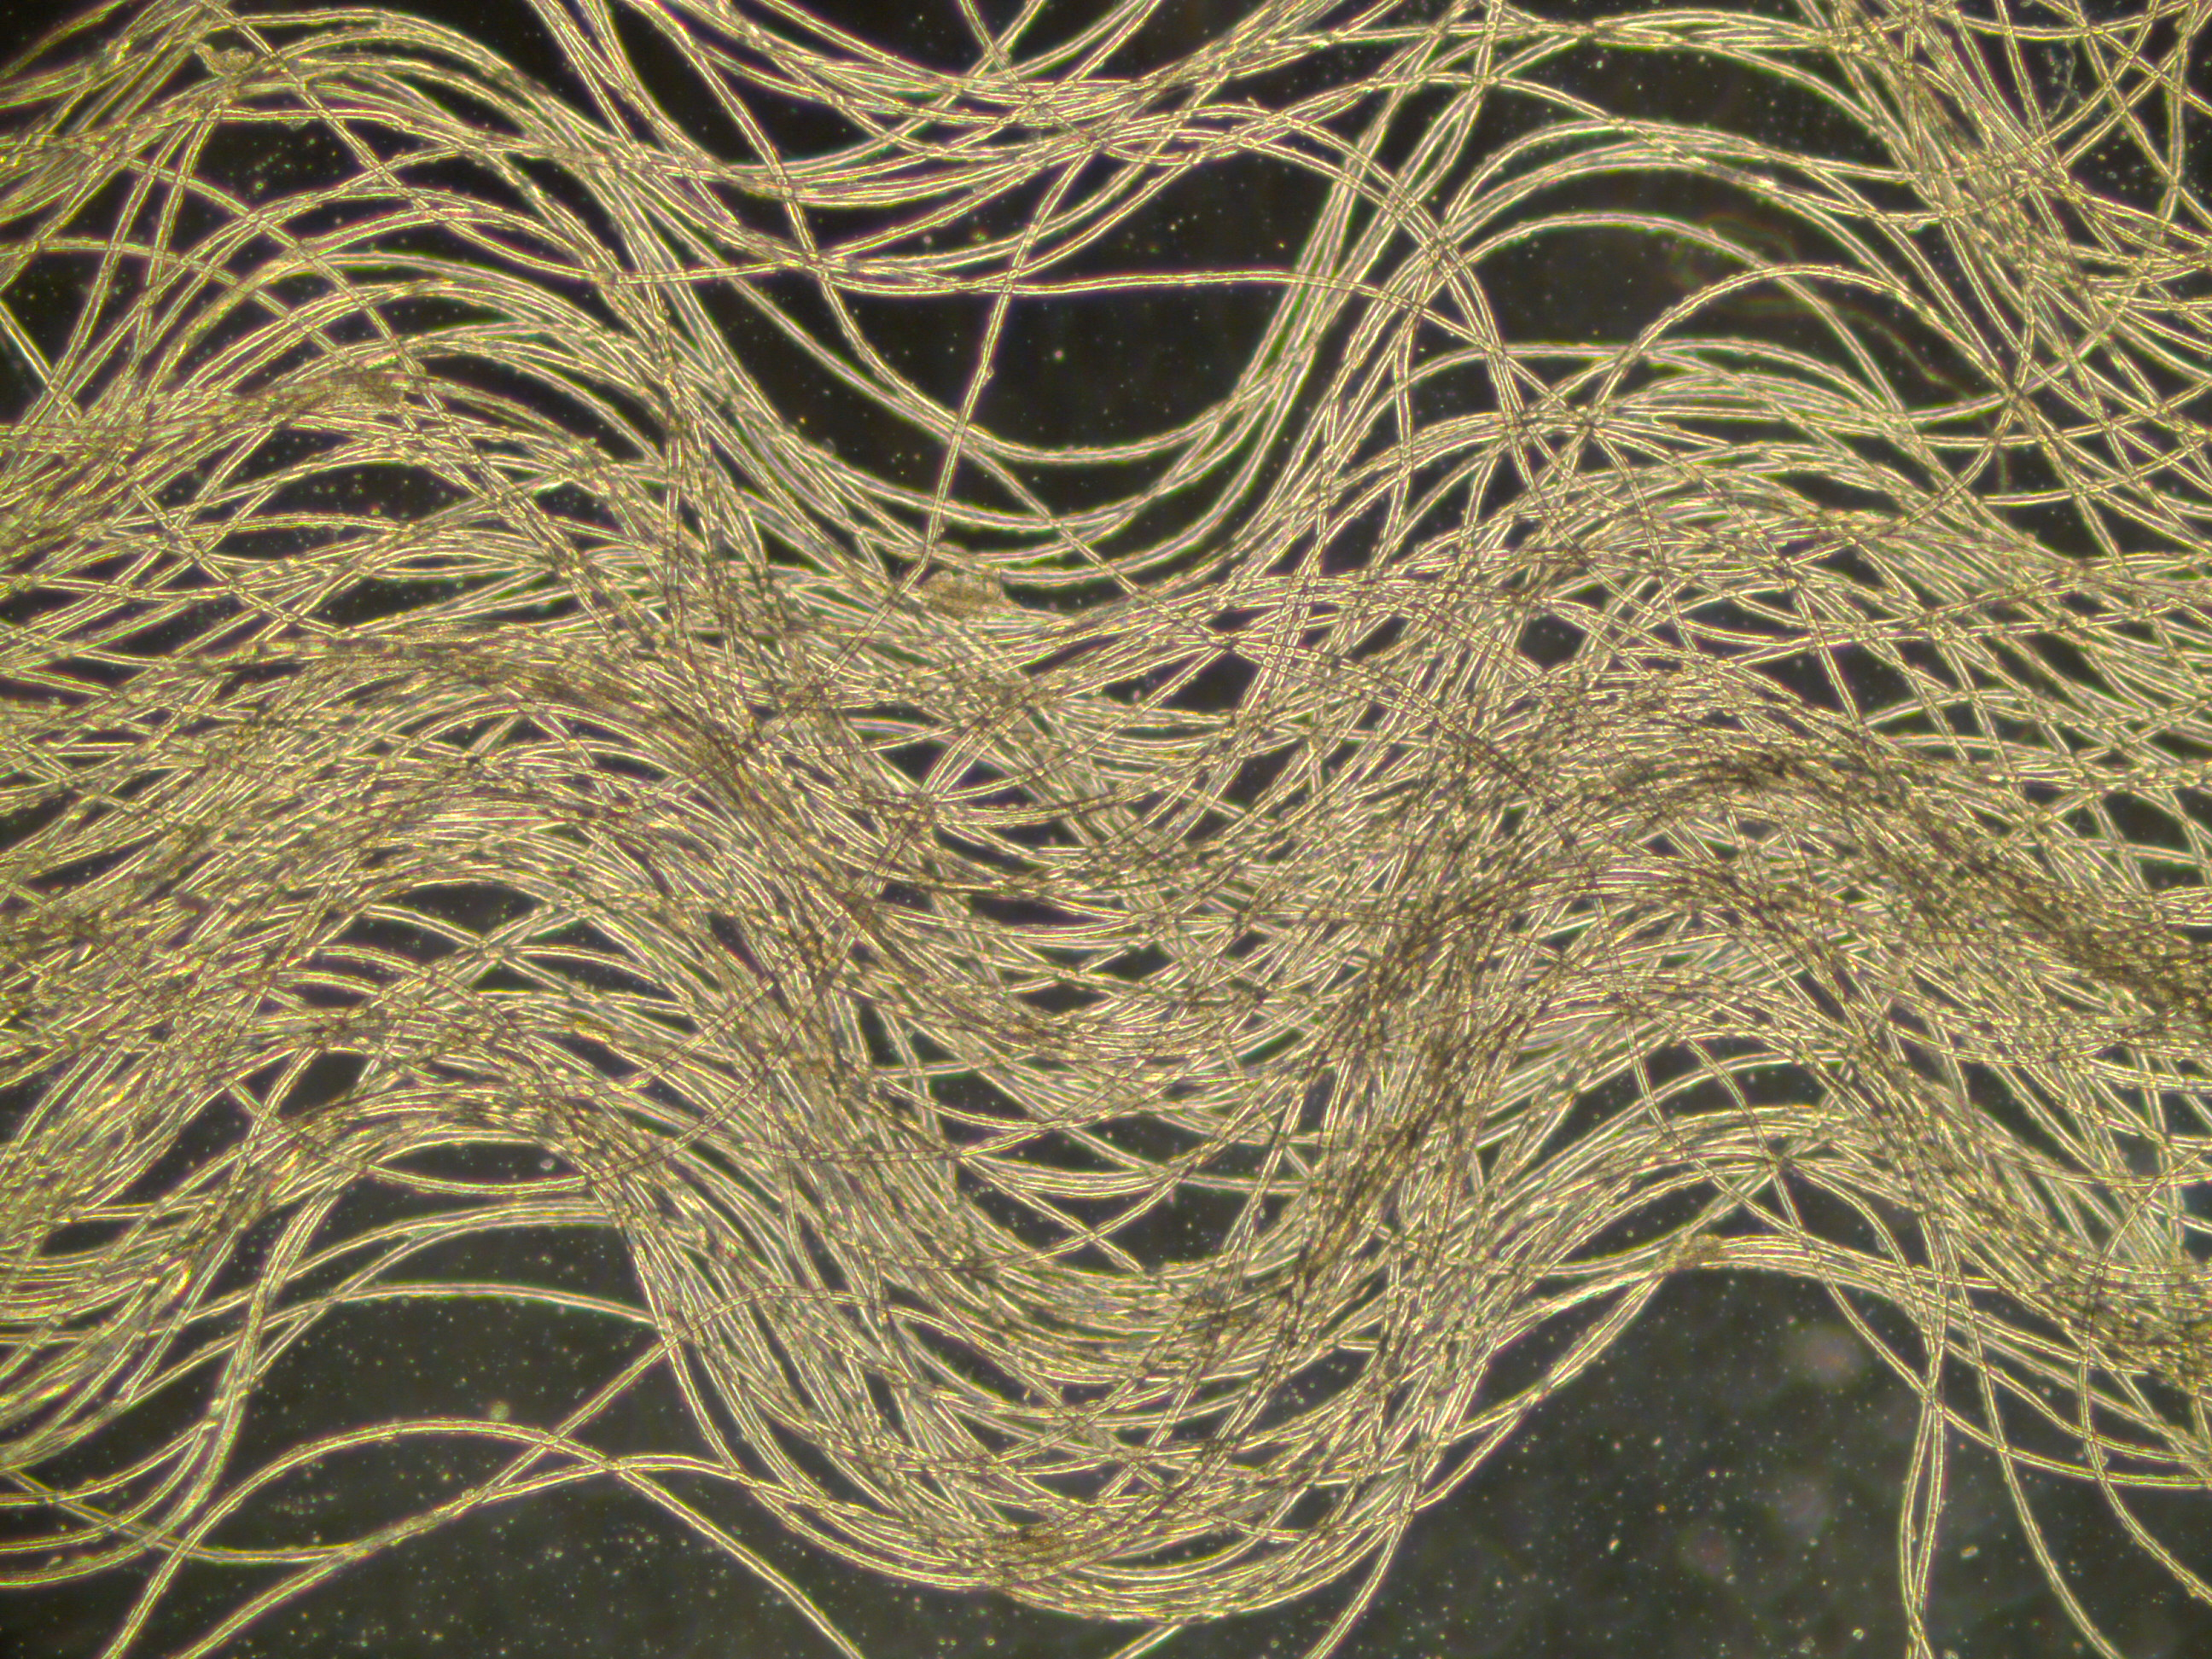
\includegraphics[width=1.0\textwidth,totalheight=2.3in]{figfibresunaligned.jpg}
    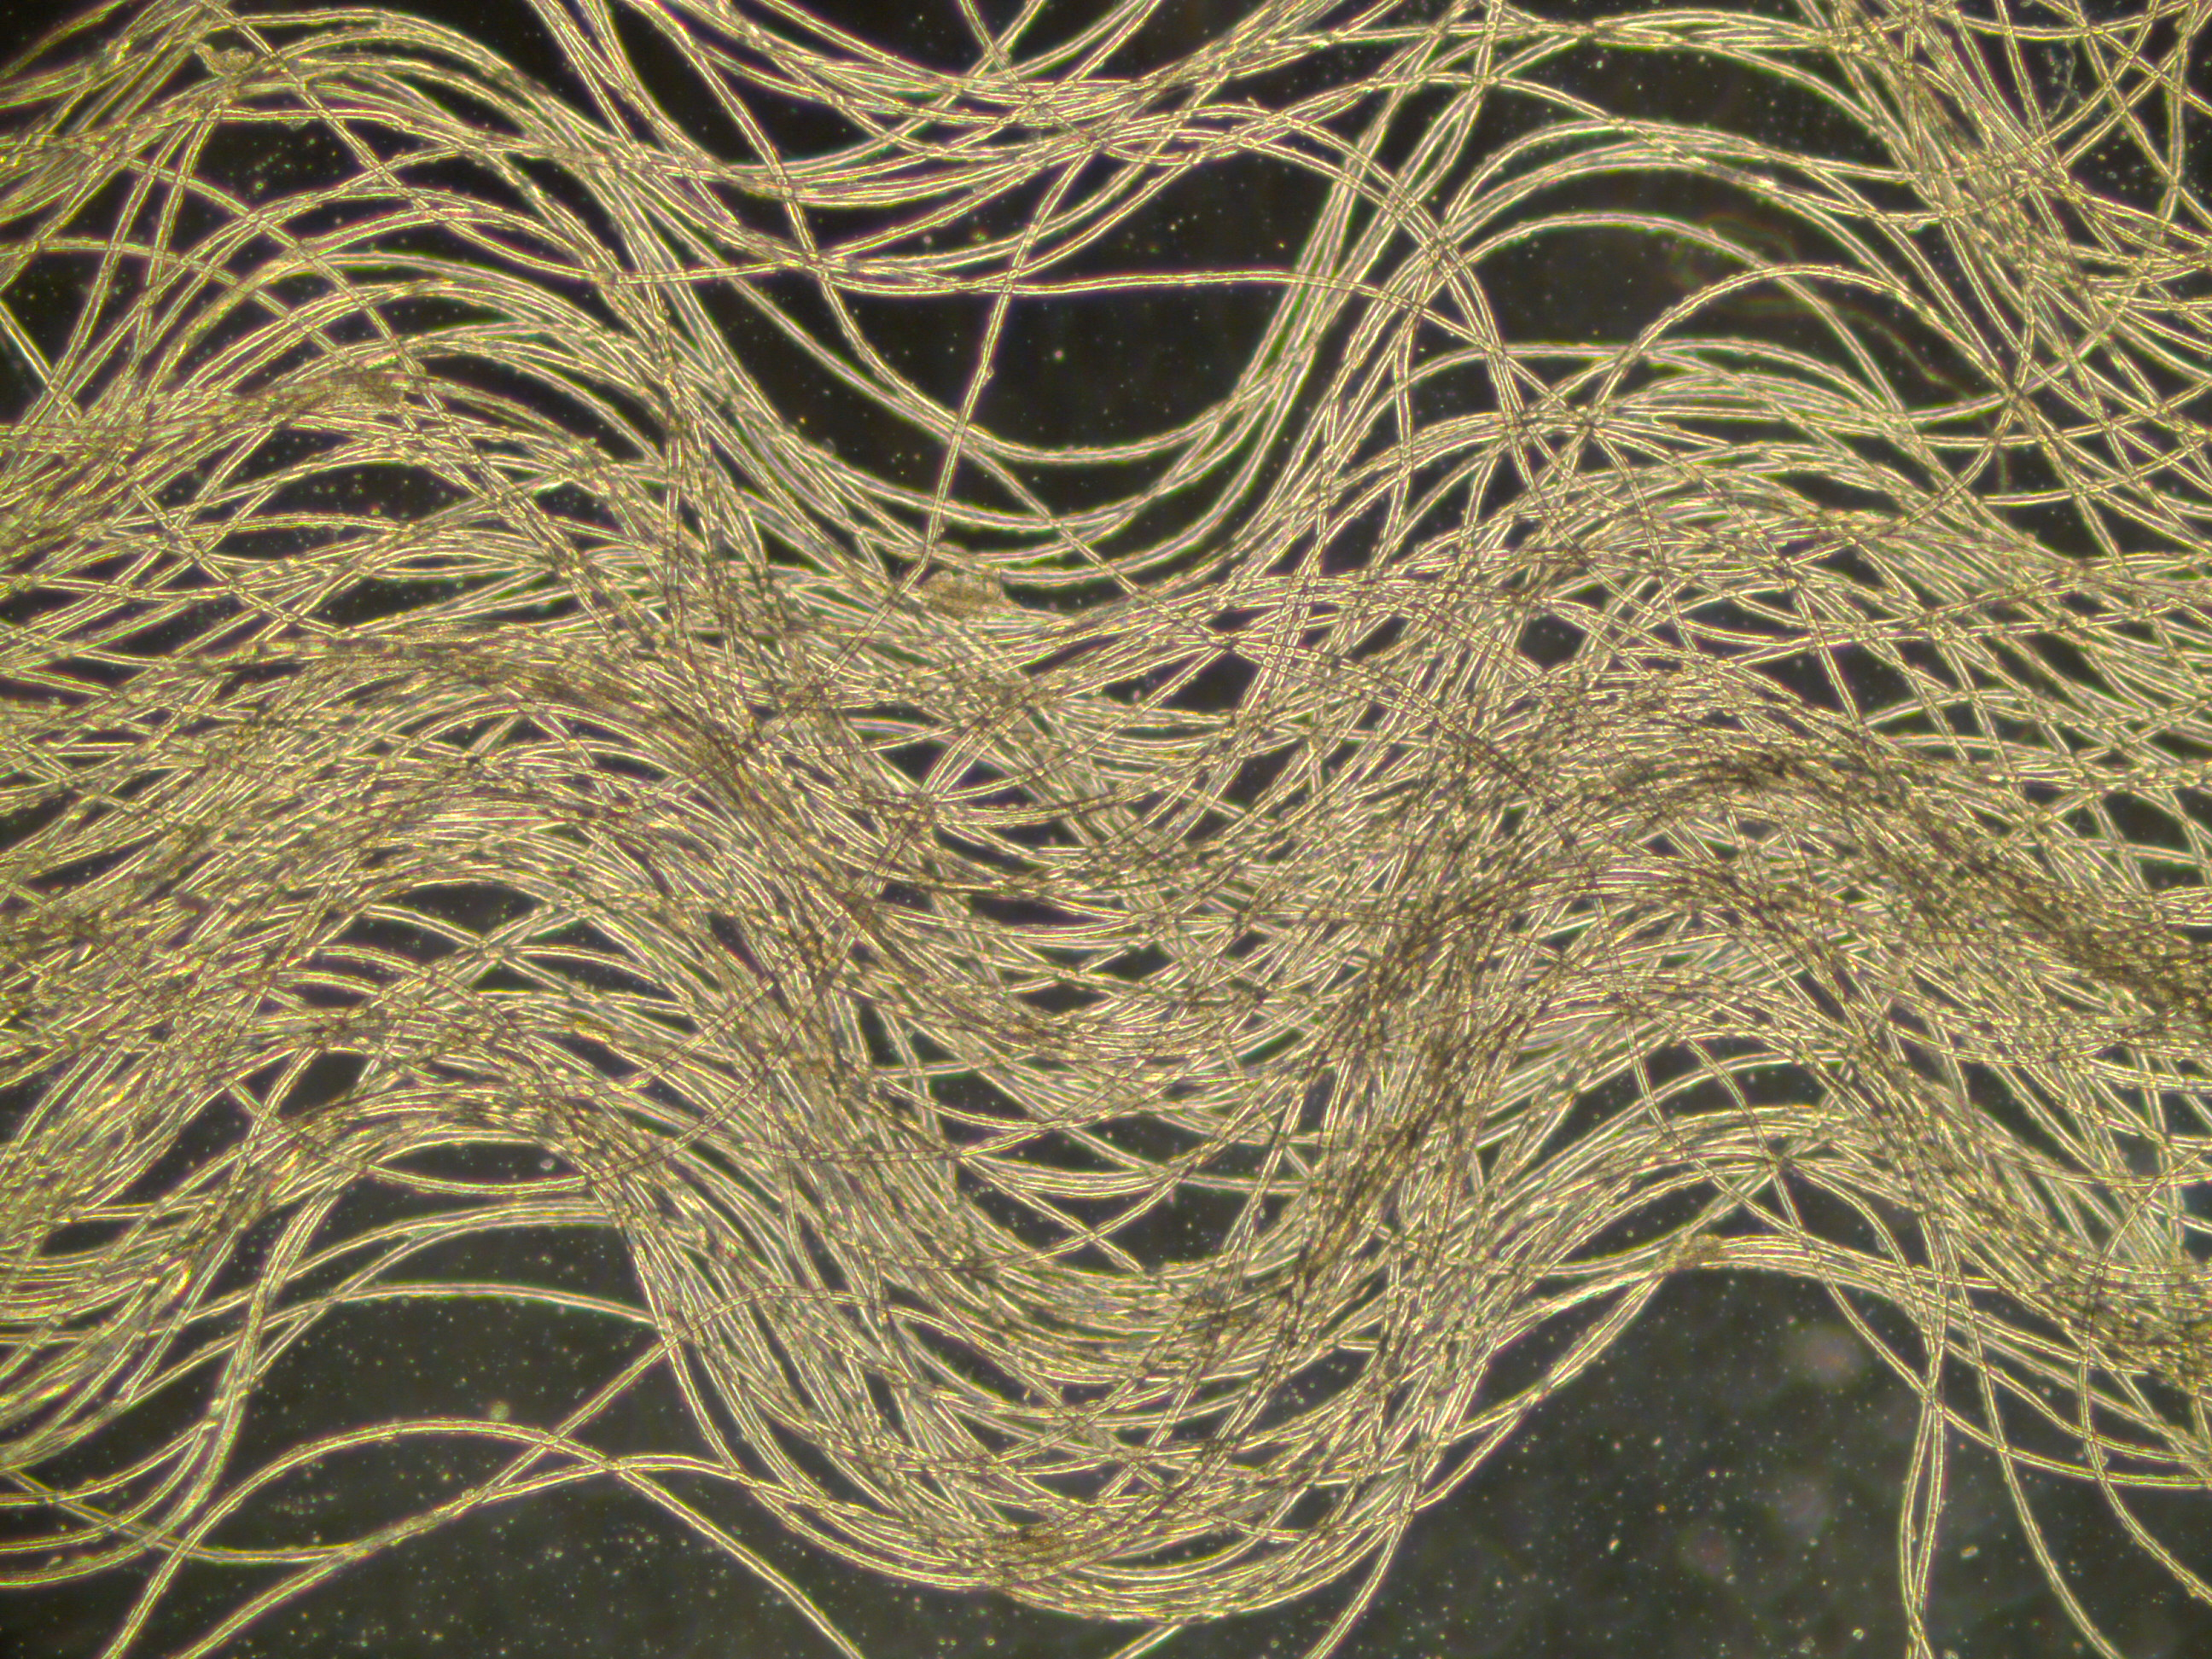
\includegraphics[scale=0.33]{figfibresunaligned.jpg}
    \label{fig:fibresunaligned}
  }

  \subfigure[{\em Stretched} staple crimp type] {
%   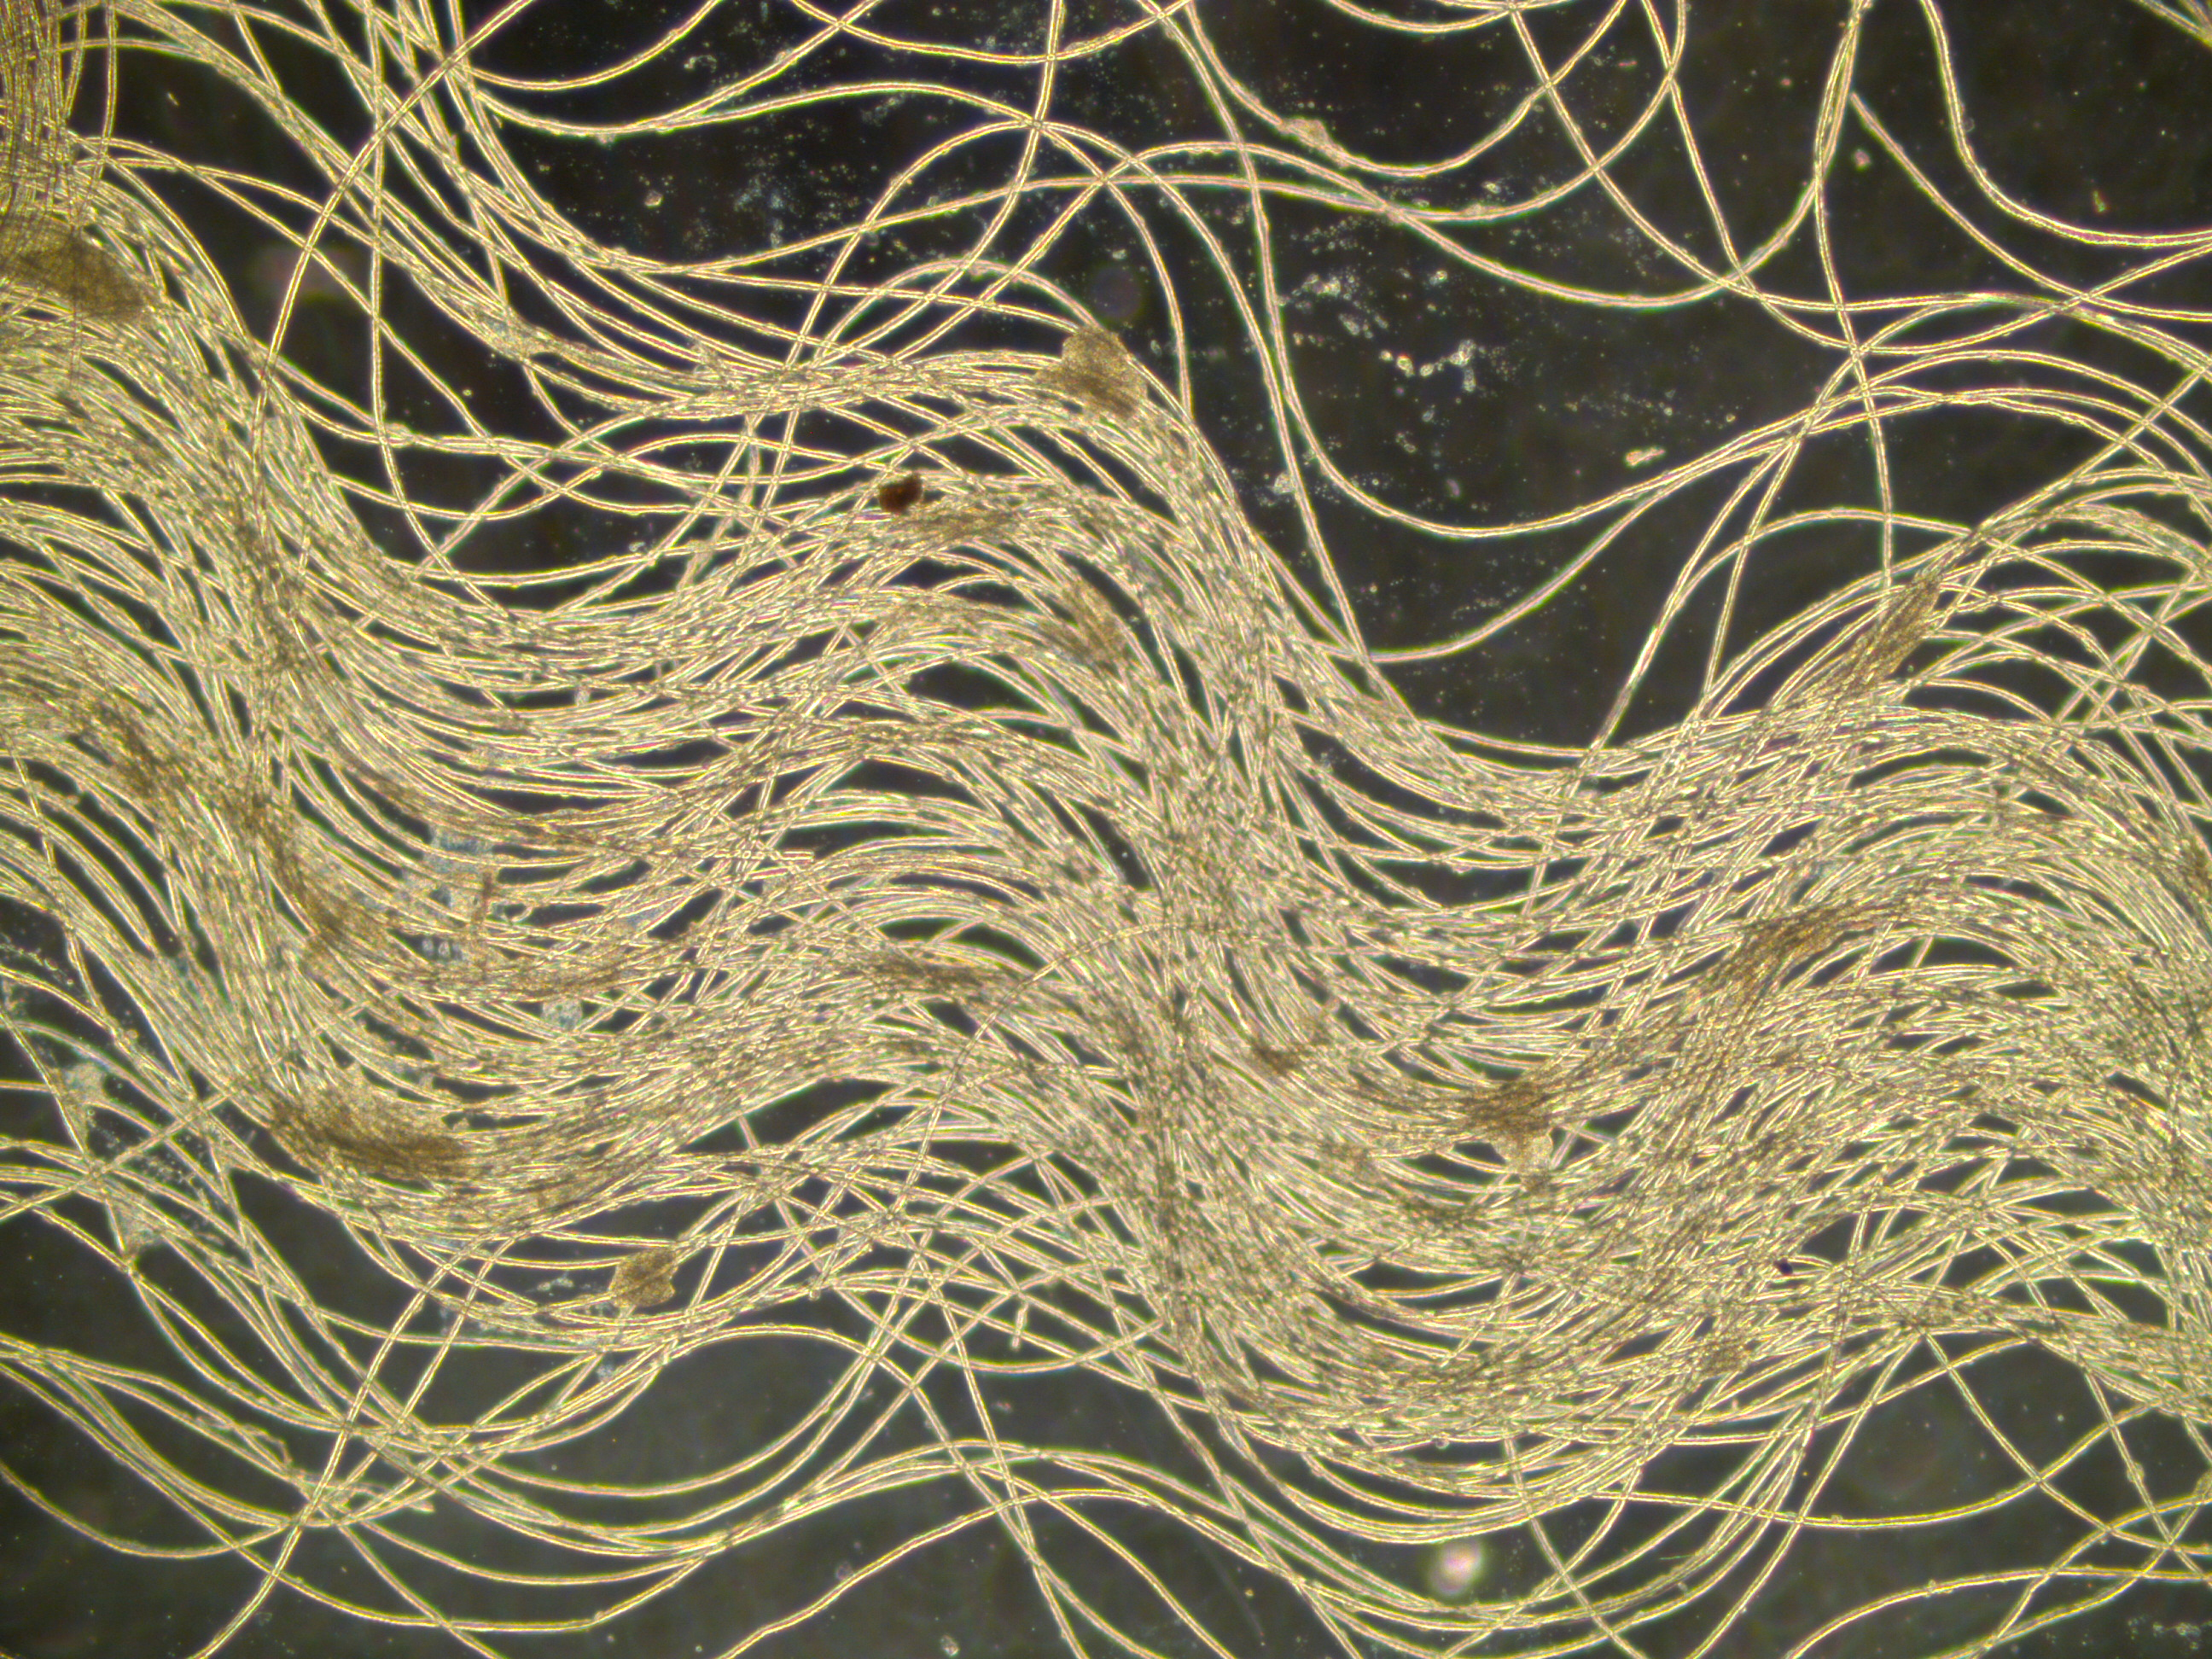
\includegraphics[width=1.0\textwidth,totalheight=2.3in]{figfibresstretched.jpg}
    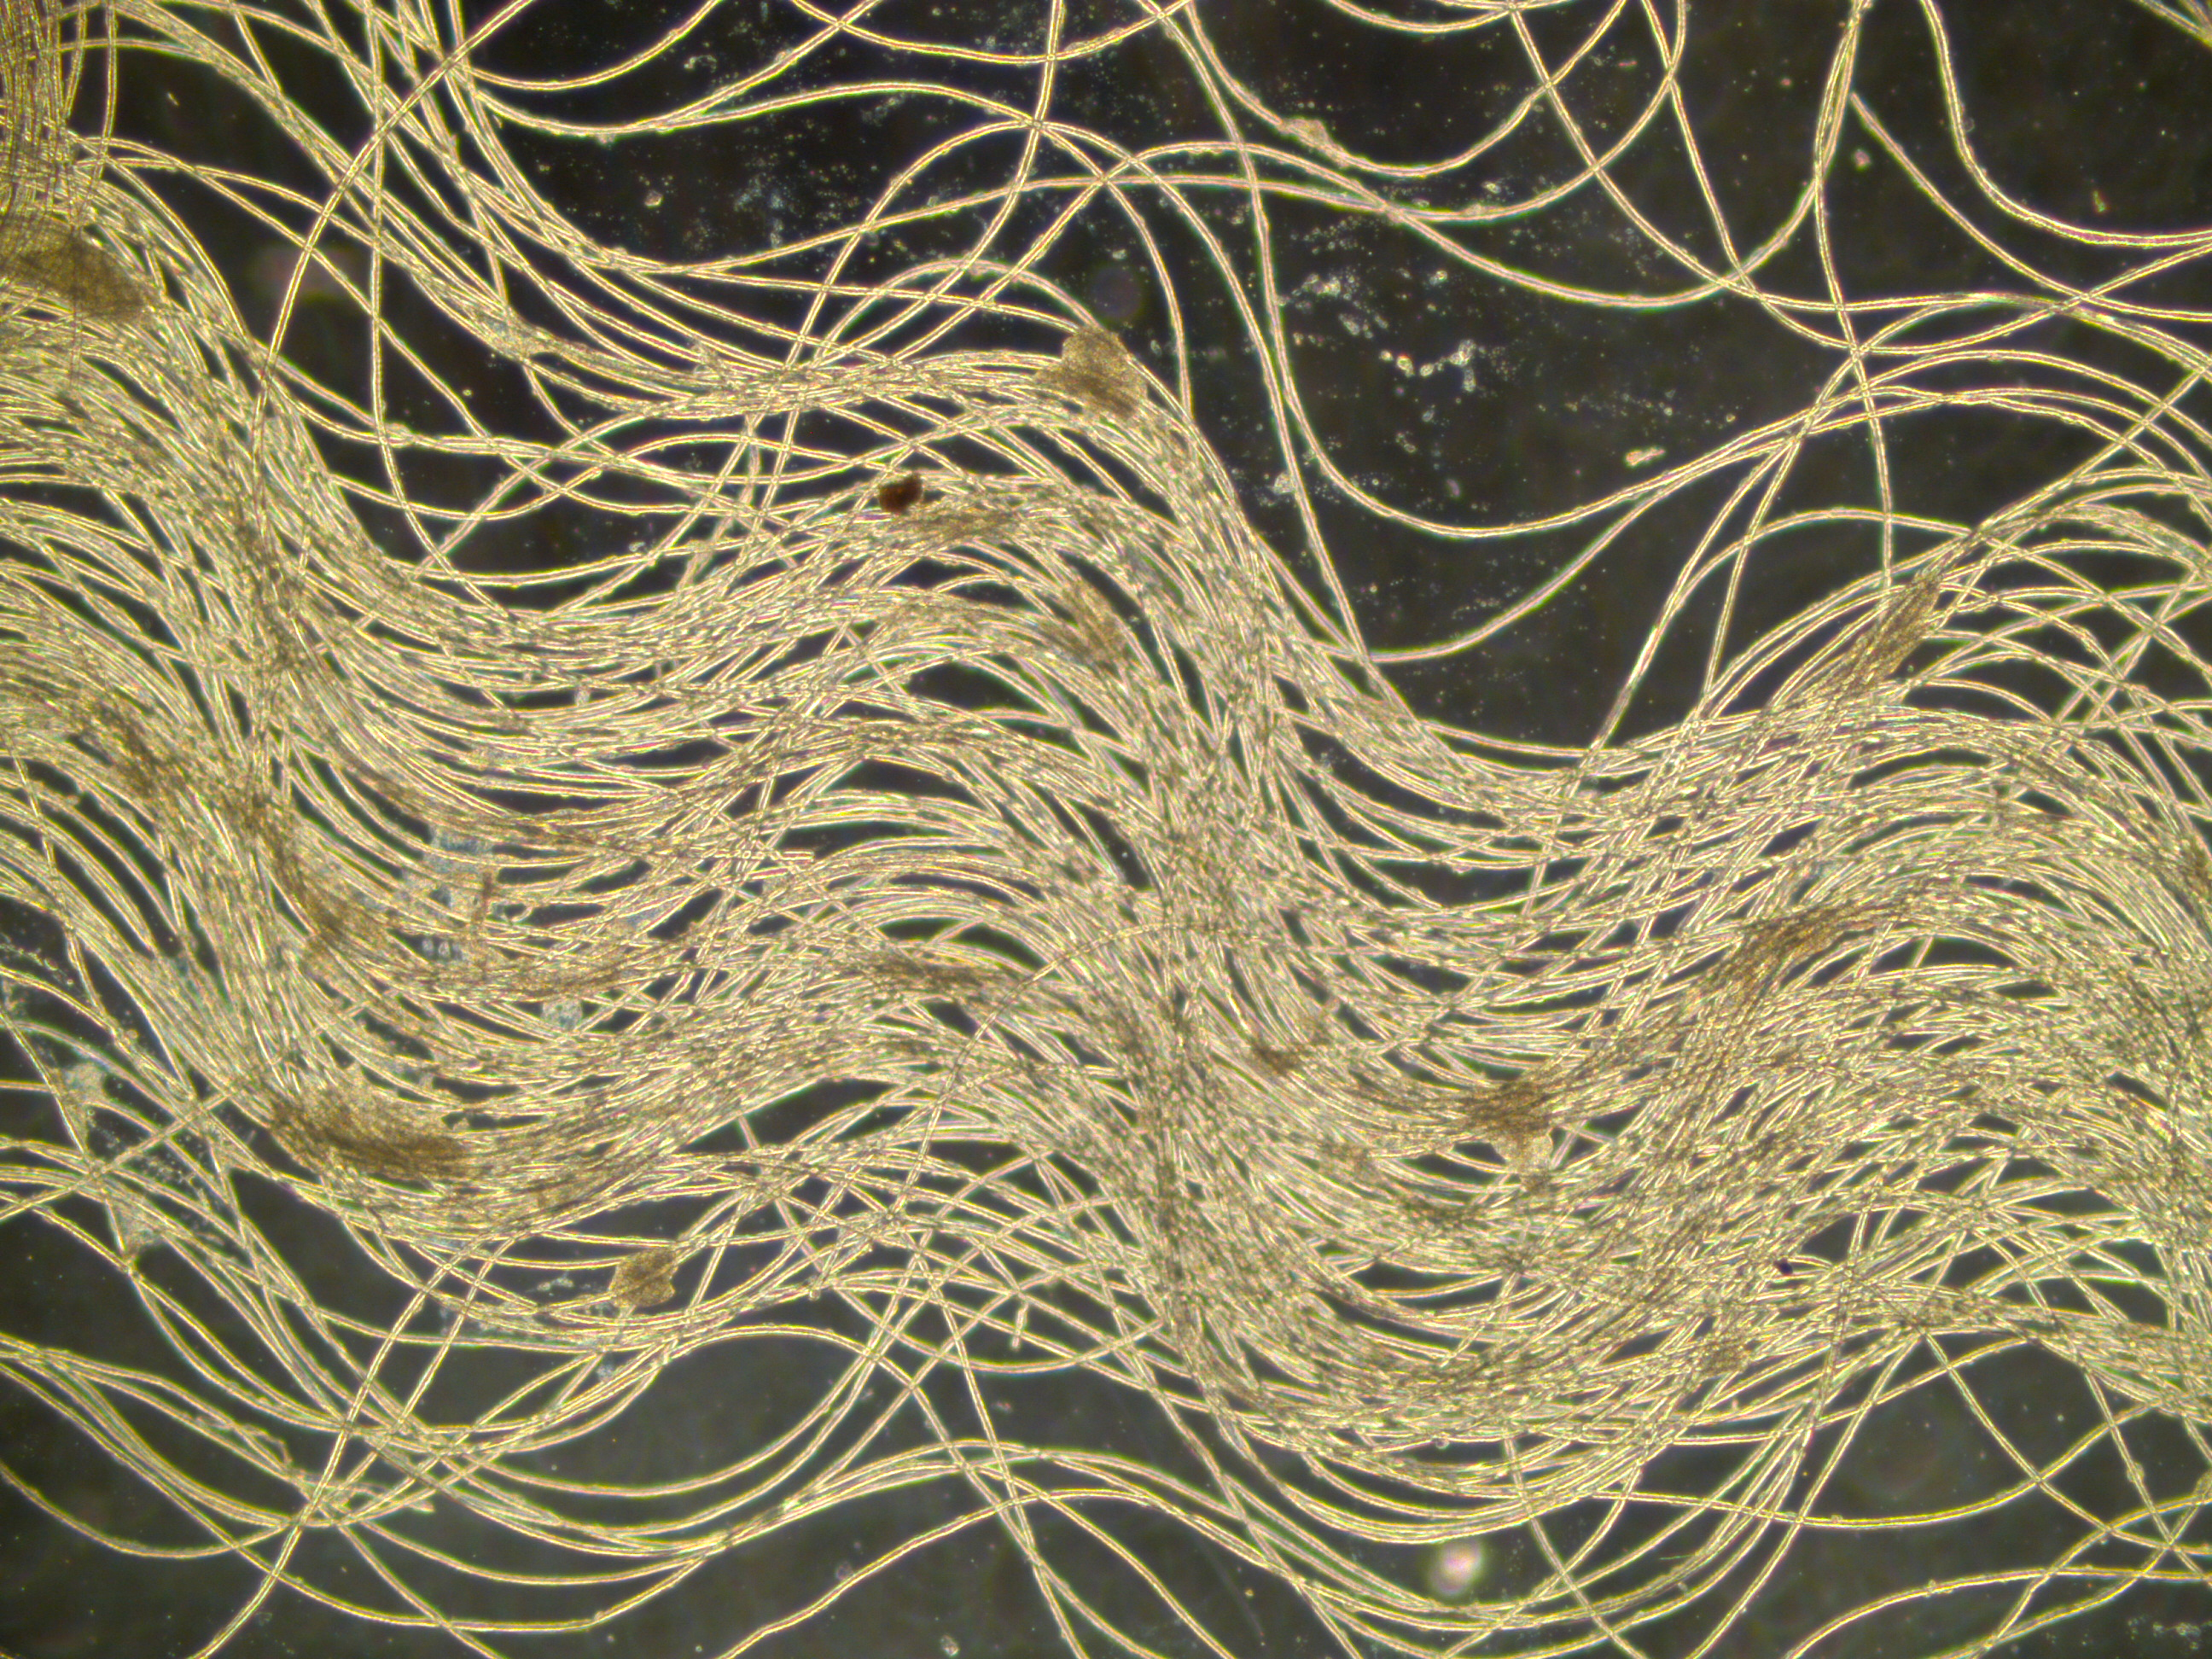
\includegraphics[scale=0.33]{figfibresstretched.jpg}
    \label{fig:fibresstretched}
  }

  \subfigure[{\em Unfolded} staple crimp type] {
%   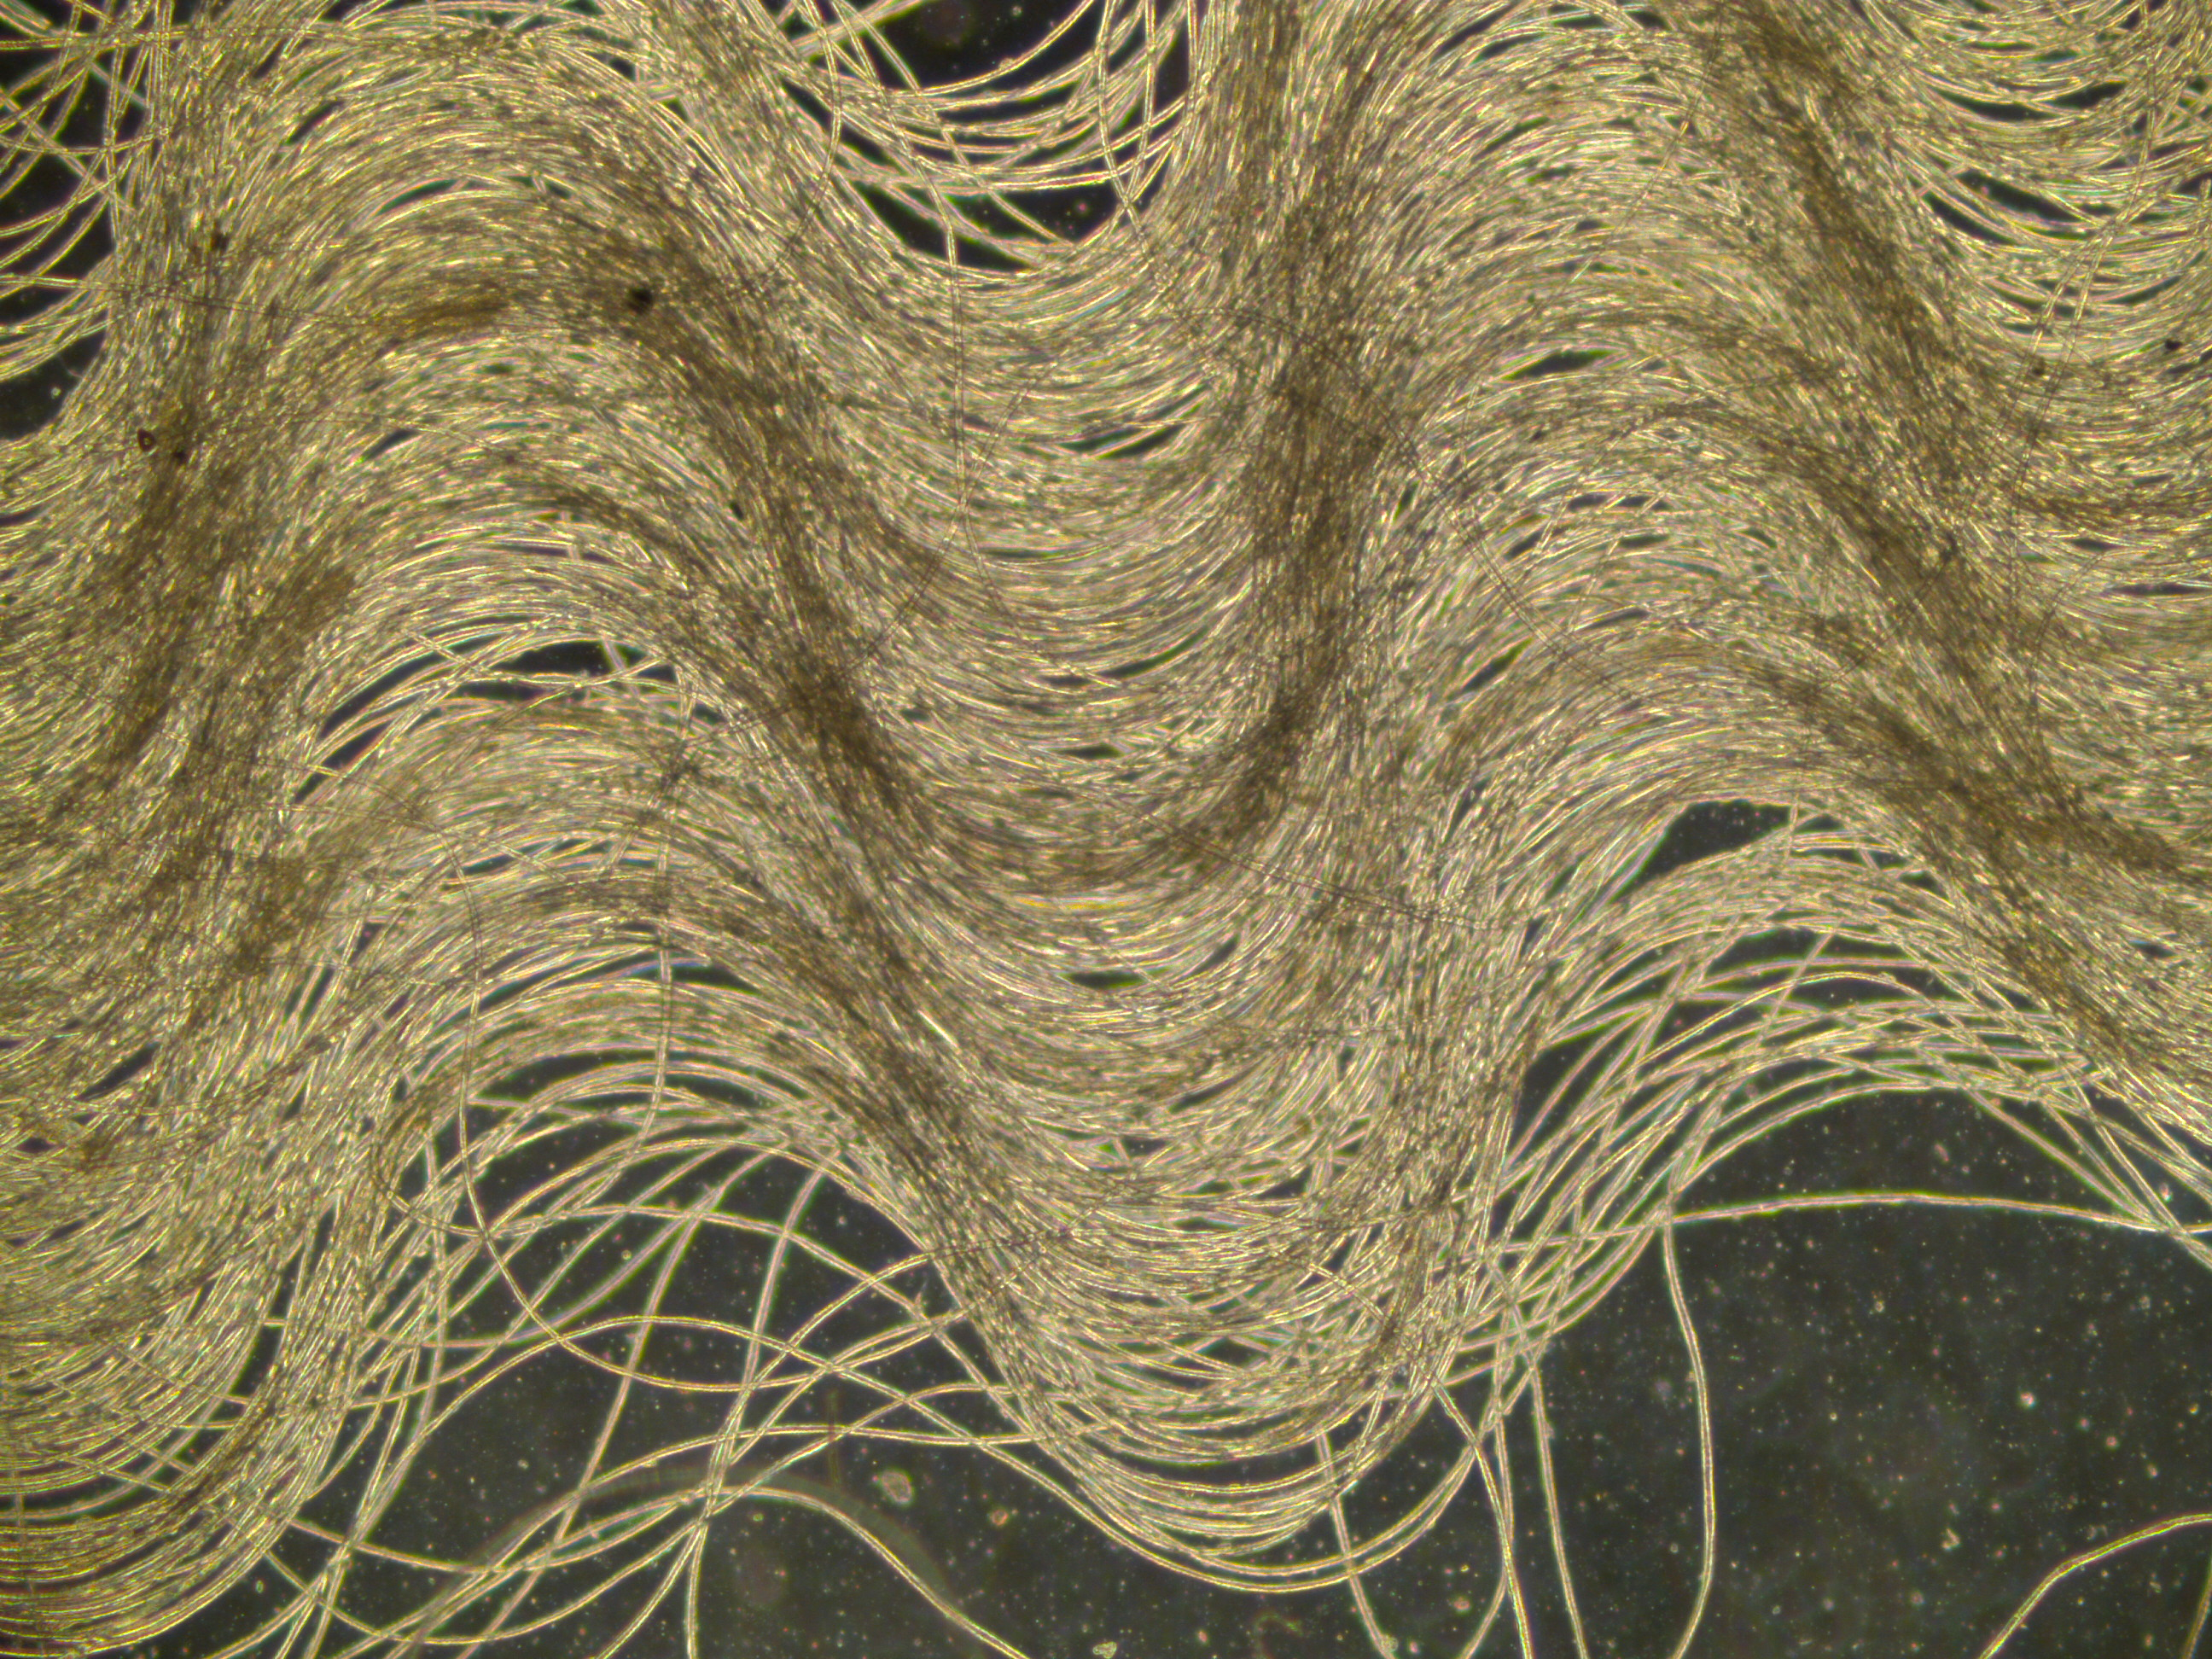
\includegraphics[width=1.0\textwidth,totalheight=2.3in]{figfibresunfolded.jpg}
    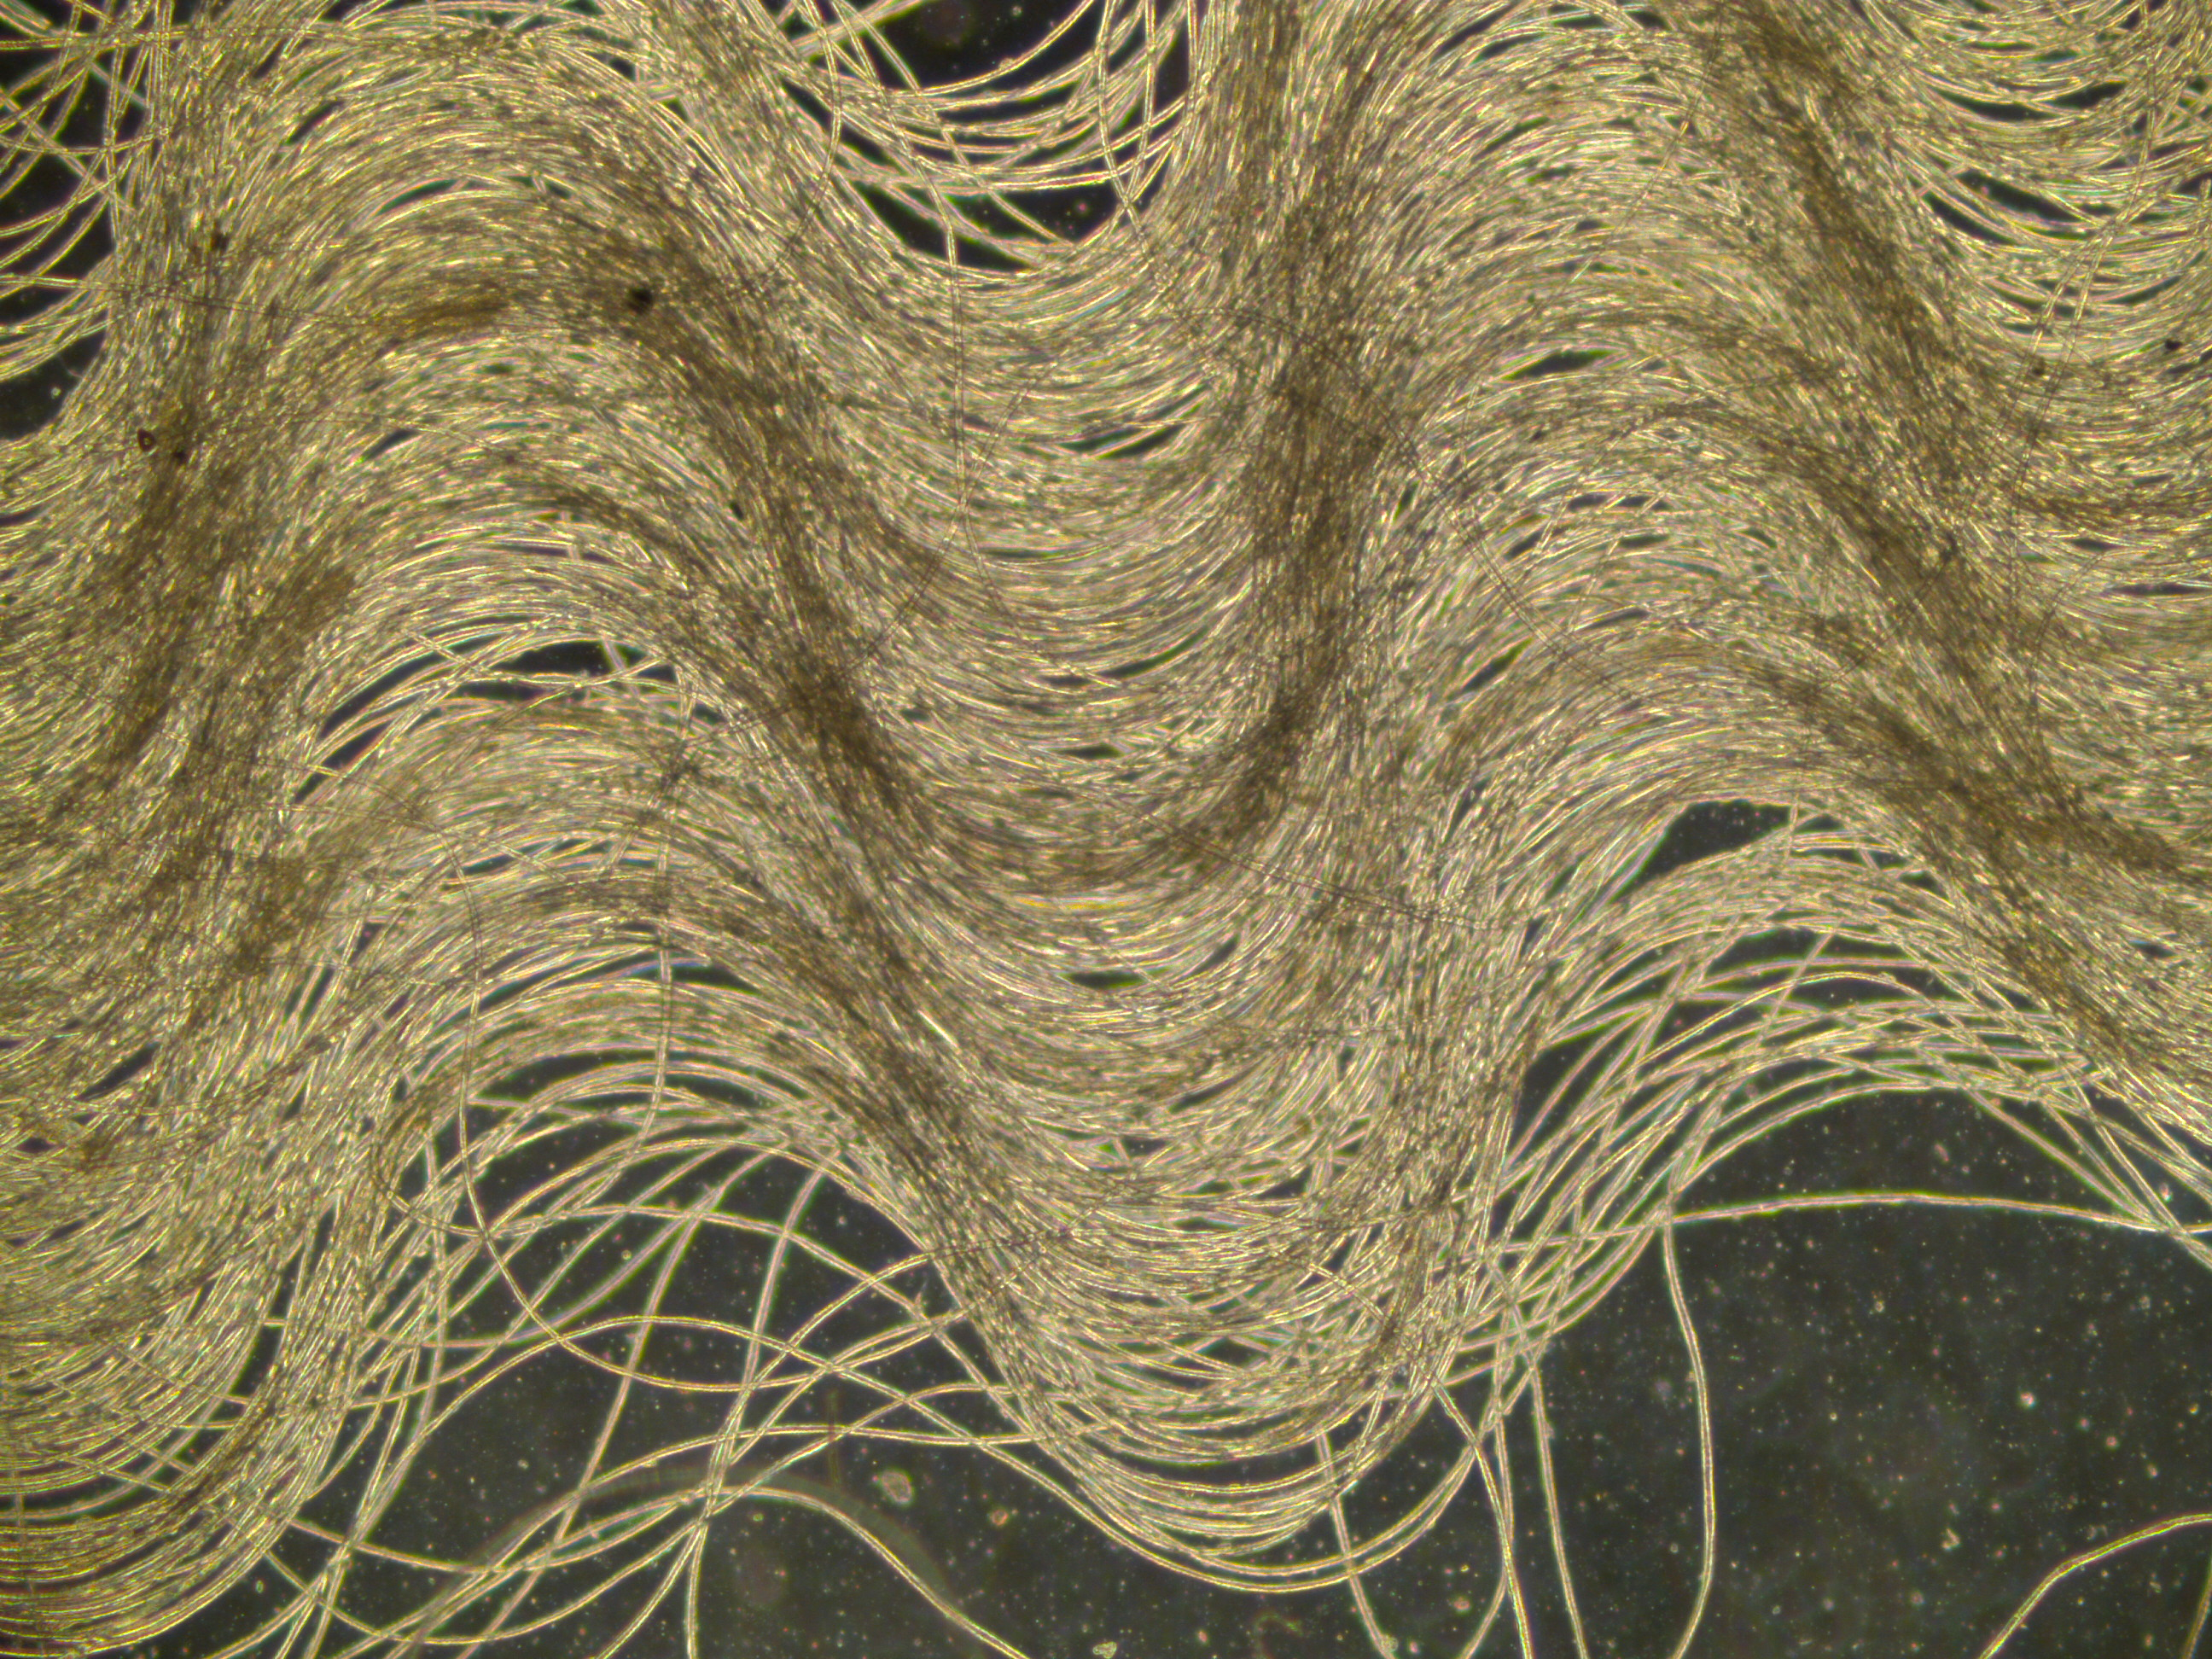
\includegraphics[scale=0.33]{figfibresunfolded.jpg}
    \label{fig:fibresunfolded}
  }

 
  \caption{Photomicrographs, taken with phase contrast microscope, showing multiple bundles of fibres for each of the three staple crimp types. Microscope magnification 25x. For printed or screen magnification see Appendix.}
  \label{fig:fibre3types}

\end{figure}

%\end{document}

